\chapter{IPv6}

\section{Representation}

IPv6 addresses are 128 bits in length and written as a string of 32 hexadecimal values. Every 4 bits is represented by a single hexadecimal digit. The preferred format for writing an IPv6 address is x:x:x:x:x:x:x:x, where each ``x'' is a single \emph{hextet}\footnote{four hexadecimal values}. For example,

\begin{verbatim}
2001:0DB8:0000:1111:0000:0000:0000:0200
\end{verbatim}

There are two rules to help reduce the number of digits needed to represent an IPv6 address.

\begin{itemize}
\item \textbf{Omit leading 0s:} Omit any leading 0s (zeros) in any hextet. This rule only applies to leading 0s, NOT to trailing 0s; otherwise, the address would be ambiguous. For example, the hextet \verb|0ABC| will become \verb|ABC|.

\begin{verbatim}
2001:0DB8:0000:1111:0000:0000:0000:0200
2001: DB8:   0:1111:   0:   0:   0: 200
\end{verbatim}

\item \textbf{Omit 0 segments:} Double colon (::) can replace any contiguous string of one or more hextets consisting of all 0s. The double colon (::) can only be used once within an address; otherwise, there would be more than one possible resulting address. 

\begin{verbatim}
2001:0DB8:0000:1111:0000:0000:0000:0200
2001: DB8:   0:1111:   0:   0:   0: 200
2001: DB8:   0:1111::200
\end{verbatim}
\end{itemize}

\section{Types of IPv6 Addresses}

There are three types of IPv6 addresses: Unicast, Multicast, and Anycast. Unlike IPv4, IPv6 does not have a broadcast address. However, there is an IPv6 all-node multicast address that essentially gives the same result.

\subsection{Unicast IPv6}

An IPv6 unicast address uniquely identifies an interface on an IPv6-enabled device. There are three types of IPv6 unicast address: Global unicast, Link-local and Unique local unicast.

\paragraph{Global unicast:} A global unicast address  is a globally unique and Internet-routable address. The ICANN\footnote{Internet Committee for Assigned Names and Numbers} assigns IPv6 Global Unicast address to organization. A global unicast address has three parts: Global routing prefix, Subnet ID, Interface ID (Figure \ref{GUA}). The \textbf{global routing prefix} (first three hextets) is the network portion of the IPv6 address that is assigned by the ISP. The \textbf{Subnet ID} (fourth hextet) is used by an organization to identify subnets within its site. The \textbf{Interface ID} (last four hextets) is the host portion of the address.

\begin{figure}[hbtp]
\caption{Global routing prefix}\label{GUA}
\centering
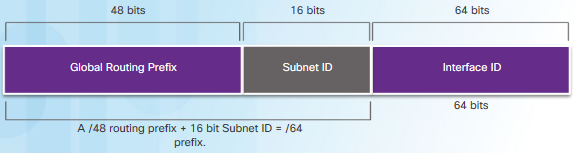
\includegraphics[scale=0.6]{pictures/GUA.PNG}
\end{figure}


\paragraph{Link-local:} Link-local addresses are used to communicate with other devices on the same local link\footnote{With IPv6, the term link refers to a subnet.}. Packets with a source or destination link-local address cannot be routed beyond the link from which the packet originated. Their uniqueness must only be confirmed on that link. If a link-local address is not configured manually on an interface, the device will automatically create its own. IPv6 link-local addresses are in the \textbf{FE80::/10} range\footnote{The /10 indicates that the first 10 bits are 1111 1110 10xx xxxx. The first hextet has a range of 1111 1110 1000 0000 (FE80) to 1111 1110 1011 1111 (FEBF)}.

\paragraph{Dynamic Link-Local Addresses} A link-local address can be established dynamically or configured manually as a static link-local address. Operating systems will typically use either EUI-64 process or a randomly generated 64-bit number to dynamically assign link-local address. By default, Cisco routers use EUI-64 to generate the Interface ID for all link-local address on IPv6 interfaces. For serial interfaces, the router will use the MAC address of an Ethernet interface.

\paragraph{Static Link-Local Addresses} A drawback to using the dynamically assigned link-local address is its long interface ID, which makes it challenging to identify and remember assigned addresses. Configuring the link-local address manually provides the ability to create an address that is recognizable and easier to remember.

\begin{verbatim}
R1(config)# interface g0/0
R1(config-if)# ipv6 address fe80::1 link-local
\end{verbatim}

The link-local address in the above example is used to make it easily recognizable as belonging to router R1. The same IPv6 link-local address is configured on all of R1's interfaces. FE80::1 can be configured on each link because it only has to be unique on that link. Similar to R1, router R2 would be configured with FE80::2 as the IPv6 link-local address on all of its interfaces

\paragraph{Unique local unicast:}Unique local addresses are used for local addressing within a site or between a limited number of sites. These addresses should not be Internet-routable and should not be translated to a global IPv6 address. Unique local addresses can be used for devices that will never need or have access from another network. Unique local addresses are in the range of \textbf{FC00::/7 to FDFF::/7}.

\subsection{Multicast IPv6}

IPv6 multicast addresses have the prefix \textbf{FF00::/8}. Multicast addresses can only be destination addresses and not source addresses. There are two types of IPv6 multicast addresses: Assigned multicast address and Solicited node multicast address.

\paragraph{Assigned mulicast addresses} are reserved multicast addresses for predefined groups of devices. For example, \textbf{FF02::1} is the all-nodes multicast address, which has the same effect as broadcast IPv4 address. The all-routers multicast address \textbf{FF02::2} identifies a group of all IPv6 routers\footnote{A router with the ipv6 unicast-routing global configuration command executed} on the network.

\paragraph{A solicited-node multicast address} is mapped to a special Ethernet multicast address. This allows the Ethernet NIC to filter the frame by examining the destination MAC address.

\section{ICMPv6}

The informational and error messages found in ICMPv6 are very similar to the control and error messages implemented by ICMPv4. However, ICMPv6 has new features and improved functionality not found in ICMPv4. ICMPv6 includes four types of message: RS and RA message\footnote{Router Solicitation (RS) message, Router Advertisement (RA) message} (communication between a router and a device), NS and NA message\footnote{Neighbor Solicitation (NS) message, Neighbor Advertisement (NA) message} (communication between devices). Address resolution and DAD process use NA and NS message, while RS and RA message contribute to assigning IPv6 to devices.\\

\begin{figure}[hbtp]
\caption{Address Resolution}\label{AddressResolution}
\centering
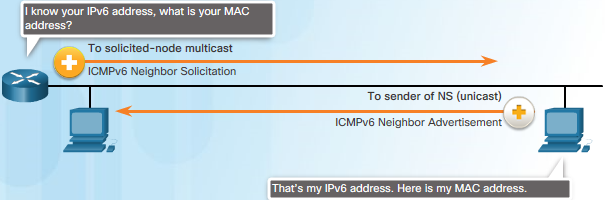
\includegraphics[scale=1]{pictures/AddressResolution.PNG}
\end{figure}


\paragraph{Address resolution} acts like ARP of IPv4. It is used to determine the MAC address of a destination IPv6 address. A device will send an NS message to the solicited node address to ask for MAC address. The message will include the known (targeted) IPv6 address. The device that has the targeted IPv6 address will respond with an NA message containing its Ethernet MAC address. Figure \ref{AddressResolution} shows two PCs exchanging NS and NA messages.

\begin{figure}[hbtp]
\caption{DAD process}\label{DADprocess}
\centering
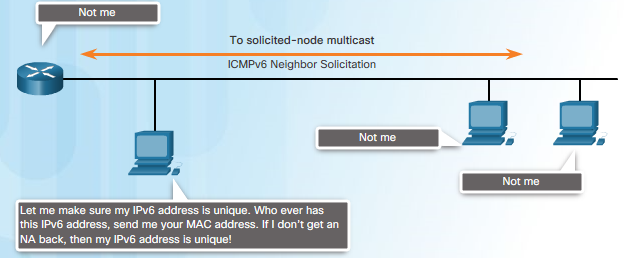
\includegraphics[scale=1]{pictures/DADprocess.PNG}
\end{figure}


\paragraph{DAD process} is a Duplicate Address Detection.  To check the uniqueness of an address, the device will send an NS message with its own IPv6 address as the targeted IPv6 address, shown in Figure \ref{DADprocess}. If another device on the network has this address, it will respond with an NA message. This NA message will notify the sending device that the address is in use. If a corresponding NA message is not returned within a certain period of time, the unicast address is unique and acceptable for use.



\section{EUI-64 Process}

When the RA message is either SLAAC or SLAAC with stateless DHCPv6, the client must generate its own Interface ID using EUI-64 Process or Randomly Generated. An EUI-64 Interface ID is represented in binary and is made up of three parts (Figure \ref{EUI64}):

\begin{itemize}
\item \textbf{24-bit OUI} from the client MAC address\footnote{Ethernet MAC addresses are made up of two parts: vendor code OUI assigned by IEEE and device identifier}, but the 7th bit (the Universally/Locally (U/L) bit) is reversed. This means that if the 7th bit is a 0, it becomes a 1, and vice versa.
\item The inserted 16-bit value \textbf{FFFE} (in hexadecimal).
\item \textbf{24-bit Device Identifier} from the client MAC address.
\end{itemize}

\begin{figure}[hbtp]
\caption{EUI-64 process}\label{EUI64}
\centering
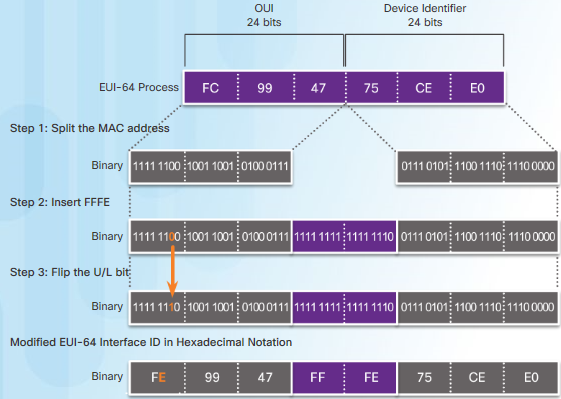
\includegraphics[scale=1]{pictures/EUI64.PNG}
\end{figure}

The advantage of EUI-64 is the Ethernet MAC address can be used to determine the Interface ID. It also allows network administrators to easily track an IPv6 address to an end device using the unique MAC address. However, this has caused privacy concerns among many users. They are concerned that their packets can be traced to the actual physical computer. Due to these concerns, a randomly generated Interface ID may be used instead. 

\section{IPv4 and IPv6 Coexistence}

Several techniques have been developed to accommodate a variety of transition IPv4-to-IPv6 scenarios:

\begin{itemize}
\item \textbf{Dual-stack:} A device interface is running both IPv4 and IPv6 protocols enabling it to communicate with either network.
\item \textbf{Tunneling:} The process of encapsulating an IPv6 packet inside an IPv4 packet. This allows the IPv6 packet to be transmitted over an IPv4-only network.
\item \textbf{Translation:} NAT64 allows IPv6-enabled devices to communicate with IPv4-enabled devices using a translation technique similar to NAT for IPv4. An IPv6 packet is translated to an IPv4 packet and vice versa.
\end{itemize}